\documentclass[conf]{new-aiaa}

\usepackage[utf8]{inputenc}
\usepackage{float}
\usepackage{graphicx}
\usepackage{amsmath}
\usepackage[version=4]{mhchem}
\usepackage{siunitx}
\usepackage{longtable,tabularx}
\usepackage{subcaption}
\setlength\LTleft{0pt} 

\title{MP3 - Hydrogen Conversion of Small Two-Stroke Engines}

\author{Arturo Saucedo}
\affil{Department of Aerospace Engineering}
\affil{University of Illinois Urbana-Champaign, Champaign, Illinois, 61820}

\author{Braden Hill and Javier Lopez}
\affil{Department of Mechanical Science \& Engineering}
\affil{University of Illinois Urbana-Champaign, Champaign, Illinois, 61820}

\begin{document}

\maketitle

\begin{abstract}
This paper outlines the otto cycle of a small two-stroke engine, the effects of powering that engine with gaseous hydrogen, and the potential impact of a hydrogen conversion kit for engines like it. We first identify a high-impact energy-conversion system to analyze from our own perspective. Then we look to the future, and, in accordance with the United Nations' Sustainable Development Goals, implement a strategy to adapt our chosen energy-conversion system for use during the rest of the coming century. The methods implement are realistic and attainable, and culminate in an artistic model representing a proposed integration in real-world personal transportation systems.
\end{abstract}

\section{Nomenclature}

{\renewcommand\arraystretch{1.0}
\noindent\begin{longtable*}{@{}l @{\quad=\quad} l@{}}
ICE  & Internal Combustion Engine \\
$\text{CO}_2$ & Carbon Dioxide \\
TDC & Top Dead Center\\
BDC & Bottom Dead Center\\
SKU & Stock Keeping Unit \\
LHV & Lower Heating Value \\
HHV & Higher Heating Value \\
RPM & Revolutions Per Minute \\
\end{longtable*}}

\section{Introduction}
\lettrine{C}{limate} change presents an irrefutable and uncomfortable truth about the relationship between humans and the planet Earth. Due to our industrial advancements over the past few centuries, we as a species have contributed over 1.5 trillion tons of $\text{CO}_2$. \cite{owidco2andgreenhousegasemissions:total} This is also in addition to our extensive reshaping of the biosphere, whereby we contribute nearly four billion tons of $\text{CO}_2$ yearly purely as a result of extensive land use change. \cite{owidco2andgreenhousegasemissions:total} Unfortunately, much of the burden associated with a changing climate falls onto the most vulnerable peoples and regions. The wealthiest countries, which have the funds, institutions, and ability to mitigate the impact of climate change are also the main drivers of it, emitting the vast majority of greenhouse gasses. All the while, the poorest and lest developed nations, which proportionally contribute far less emissions on a global scale, often times lack the resources necessary to mitigate the impact of climate change within their borders.

This lopsided relationship between wealth and emissions leads to conflict and resentment when it comes to international efforts to curtail climate change. It is no secret that the path to success of the global north is marked with the extensive exploitation of natural and human resources, and centuries of industrial development which polluted the Earth to no end. And so, developing nations find themselves in a precarious situation; to improve their living conditions and protect against the effects of climate change, they must rapidly develop and industrialize, however in doing so they contribute to the acceleration of climate change. Finding solutions that would help less developed nations of the world progress in an environmentally-friendly way at low cost has been and continues to be at the forefront of engineering and scientific efforts across the world.

To this end, we have identified one potential solution - the conversion of small two-stroke Otto cycle engines to operate on a hydrogen-air mixture, fueled by local electrolysis operations. According to Ritchie and Roser, road transport accounts for nearly 12 percent of the global total, making it a good target for decarbonization and transition to green energies. \cite{owidco2andgreenhousegasemissions:by_sector} Figure \ref{fig:emissions_pie}, provided by Ritchie and rose, visualizes their data, putting into context the scope of the problem at hand. While the combustion of hydrogen offers lower efficiencies when compared to a hydrogen fuel cell or other green transportation technologies, it offers unique advantages which make it suited to our application. Primarily, converting small ICE systems to operate on hydrogen and air reuses already existing resources. Sometimes we as engineers and scientists get so caught up in searching for the most efficient solution to a problem that we forget to think about the most effective solution. Instead of creating further pollution and spending large sums of money in the production and procurement of brand new systems, our proposal focuses instead on using as much of existing small ICE systems as possible. Such engines are prevalent in the targeted less-developed nations, particularly in very dense regions of Asia, according to WorldAtlas \cite{motorbike}. In these regions, small two-stroke Otto cycle engines are in heavy use, and a conversion system would allow billions to keep their vehicles and eliminate their emissions at low cost. This avoids expensive hydrogen fuel cells or electric motors and their accompanying batteries. Additionally, this solution does not require advanced materials engineering technologies, such as those required for high-efficiency fuel cells. At most, this system requires knowledge on the operation of small engines, as well as knowledge and distribution of Stirling engine electric generators for local hydrogen and oxygen production. These factors combined dramatically lower the knowledge barrier of such a system, as well as the cost barrier of creating zero-emission vehicles.



\begin{figure}[hb!]
    \centering
    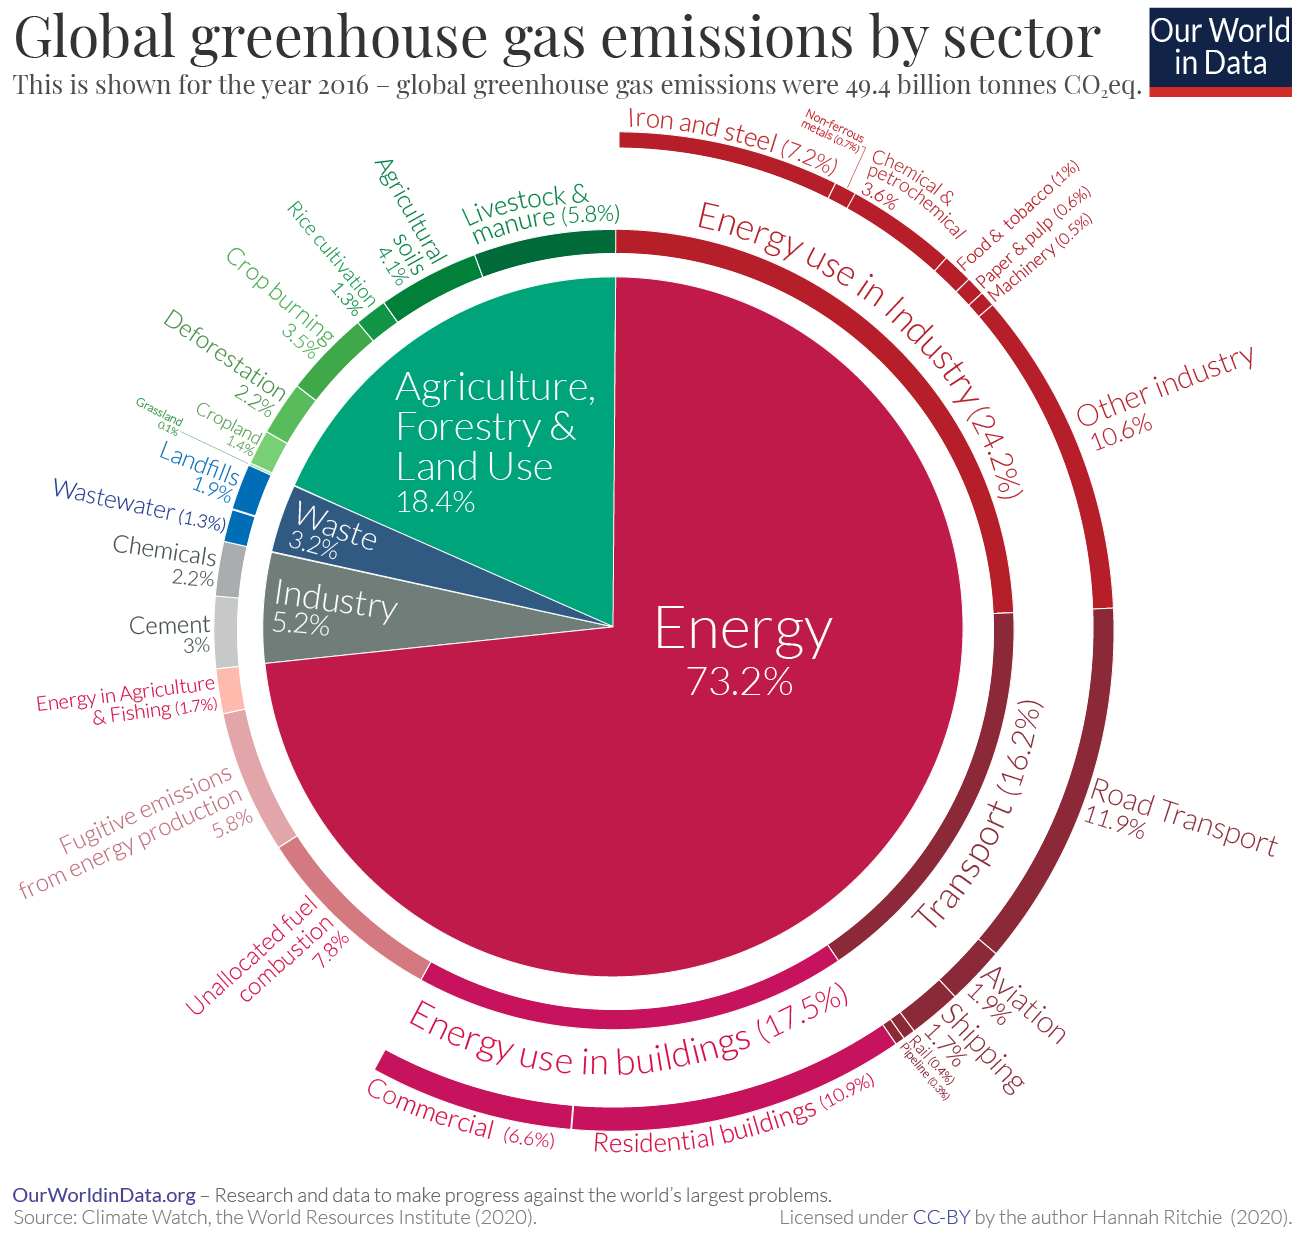
\includegraphics[width=0.8\textwidth]{Figures/pie_chart.png}
    \caption{Global greenhouse gas emissions by sector, courtesy Ritchie and Roser.\cite{owidco2andgreenhousegasemissions:by_sector}}
    \label{fig:emissions_pie}
\end{figure}

\section{Electrolysis}

\subsection{Basic Principles}
Electrolysis, in its most basic sense, is the process whereby electrical energy is applied to water to split the molecules into pure hydrogen and oxygen. For each mole of water that is electrolyzed, two moles of hydrogen and one mole of oxygen are produced. This process requires a steady input electrical energy dependent on the thermal energy already present in the water. According to Carl R. Nave of the Department of Physics and Astronomy at Georgia State University, the total electrical energy required is equal to the change in Gibbs free energy \cite{GSU}. This, in turn, depends on the change in enthalpy and the energy obtained from the environment. That is to say that given more energy from the environment, such as thermal energy, the required electrical energy decreases. This is beneficial for many applications, such as an electrolysis system using the electrical and waste heat energy from a power generation device, as discussed in the next section. A diagram created by Carl R. Nave is shown in Figure \ref{fig:electro} illustrating the water electrolysis process.

\begin{figure}[H]
    \centering
    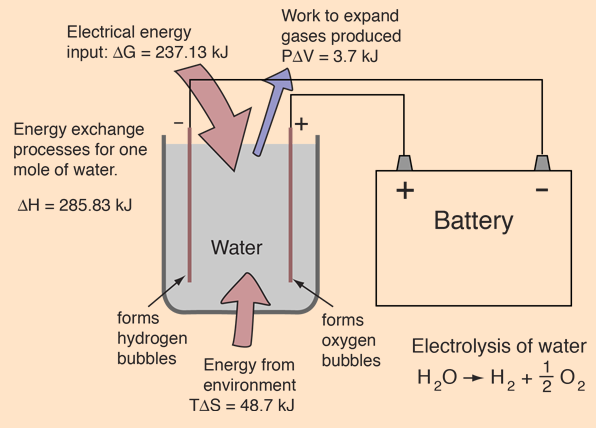
\includegraphics[width=0.8\textwidth]{Figures/GSU.PNG}
    \caption{Electrolysis diagram, courtesy Carl R. Nave, GSU. \cite{GSU}}
    \label{fig:electro}
\end{figure}



\subsection{Energy Sources}
In areas with more scarce energy generation options, a combined heat engine and electrolyzer system could be used to generate hydrogen with minimal grid demand. The use of a Stirling engine represents one such solution applicable for this system. Electrolysis would be conducted using the electrical energy of the Stirling engine, which generates that energy from an array of solar concentrators creating a heat energy differential within the engine. One frequent drawback Stirling engines face is the need for some sort of cooling to maintain the heat energy differential within the engine. However, we can cool the Stirling engine with water that would be destined for electrolysis. This arrangement would be able maintain a heat differential within the Stirling engine and transfer what would be waste heat into the water. This would reduce the electrical energy required to separate hydrogen and oxygen, improving the efficiency of both the Stirling engine and the electrolysis process. The produced gases are stable when separated and may be collected and used when necessary, with minimal concern for gas losses over time in a sealed system. Importantly, such a proposed system of solar concentrators, Stirling engines, and electrolyzers is not new tehcnology, and could be readily implemented in most regions of the world. To this end, it would simply be a matter of distributing the systems, and reducing their cost and complexity. An example of an industrial sized solar concentrator and Stirling engine setup is shown in Figure \ref{fig:stirling}.

\begin{figure}[H]
    \centering
    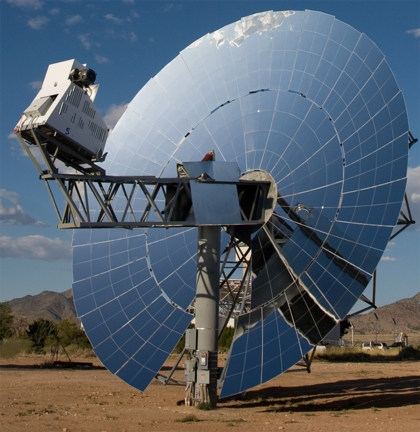
\includegraphics[width=0.6\textwidth]{Figures/stirling.jpg}
    \caption{Stirling engine powered by a solar concentrator.}
    \label{fig:stirling}
\end{figure}


\pagebreak

\section{ICE Principles of Operation}
\subsection{Otto cycle}
Ideal internal combustion engines operate by compressing a gaseous fuel and oxidizer mixture, combusting it, expanding it, and exhasusting the combusted mixture. This process generates work, and is mainly dependent on the energy generated from the combustion in the form of temperature. Many cycles are used in internal combustion engines, the most popular being the Diesel and Otto cycles. For our purposes, we will focus on the Otto cycle, due to its popularity in small personal motorized vehicles.
The Otto cycle is extensively used in spark-ignition internal combustion engines. It sees wide applications in the transportation sector, including personal ground transportation. As seen in Figure \ref{fig:otto_cycle}, the Otto process intakes air, compresses it, combusts it at constant volume (typically with the help of a spark plug in real-world applications), expands it, and finally rejects heat by expelling the combustion gasses.

The ideal Otto cycle can be summarized as follows:
\begin{enumerate}
  \item Isentropic Compression
  \item Isovolumetric Heat Addition
  \item Isentropic Expansion
  \time Isovolumetric Heat Rejection
\end{enumerate}

\begin{figure}[H]
    \centering
    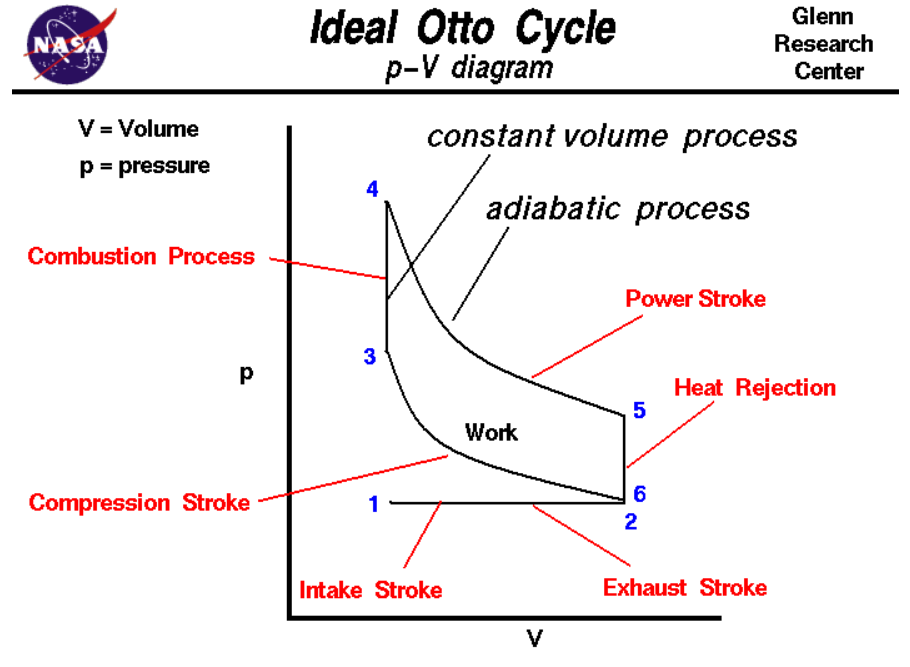
\includegraphics[width=0.6\textwidth]{Screenshot 2023-04-24 170054.png}
    \caption{General Idealized Otto Cycle, courtesy NASA.\cite{nasa_otto}}
    \label{fig:otto_cycle}
\end{figure}


\subsection{Two-Stroke}
The two-stroke combustion engine functions via an expansion and compression stroke.  The expansion stroke involves the piston descending from TDC or top dead center, its highest vertical displacement in the cycle, and in the process drawing the fresh air-fuel mixture into the cylinder while allowing the combusted gases to evacuate.  The compression stroke starts when the piston begins ascending from BDC or bottom dead center and causes the air-fuel mixture to compress in the cylinder until near-TDC is achieved, at which point a spark-plug ignites the mixture in a petrol engine or compression-ignition occurs if it is a diesel system.
\subsection{Our Engine}

The engine used in our mock-up is an 80 cubic centimeter displacement 2-stroke petrol fueled carburetor operated bicycle mountable engine.  It is a common and inexpensive mass-produced generic unit sharing similarities with many other SKUs of powered bicycle conversion kits. It is a part with wide availability across the world. This particular engine was rescued from Mack's Twin City Recycling. It did not work at first, but after some diagnosis we discovered that the carburetor was very dirty, impeding operation, as seen in Figure \ref{fig:carb}. After disassembly and cleaning, the engine was able to run on its own power for a few seconds. We attached it to a test stand for testing, pictured in Figure \ref{fig:test_stand}. Additionally pictured in Figure \ref{fig:air_intake} is the original air intake, something which would have to be replaced or adapted to feed off of pressurized air and hydrogen tanks.

\begin{figure}[H]
    \centering
    \includegraphics[width=0.8\textwidth]{Figures/carb.JPG}
    \caption{Culprit for original engine malfunction. The carburetor was full of debris. We cleaned it and placed it back on the engine, allowing for operation on two-stroke fuel.}
    \label{fig:carb}
\end{figure}

\begin{figure}[H]
    \centering
    \includegraphics[width=0.8\textwidth]{Figures/DSC_0142.JPG}
    \caption{Original air intake for the engine.}
    \label{fig:air_intake}
\end{figure}

\begin{figure}[H]
    \centering
    \includegraphics[width=0.8\textwidth]{Figures/engine_test_stand.JPG}
    \caption{Our rescued engine on its test stand, comprised of a metal pipe bicycle rack.}
    \label{fig:test_stand}
\end{figure}



\subsection{Gasoline vs Hydrogen}
\subsubsection{Comparison}
Gasoline, the combustive component of which is iso-octane, is used in internal combustion engines and detonates via the firing of a spark-plug that provides sufficient impetus to combust the compressed air-fuel mixture found inside the cylinder. The balanced chemical equation forIso-octane and air combustion is given in Equation \ref{eq:combust_iso}. This combustion inherently produces carbon dioxide emissions, which are detrimental to the environment. Hydrogen gas, naturally found as H2, can be similarly mixed with air to provide a combustible mixture for use in an engine cylinder, but has the massive, and pertinent to our study, advantage of its only chemically derived product being water.  However, current infrastructure for the storage and supply of hydrogen to consumers for transportation powering purposes is limited, and is the largest inhibitor to progress in the space.

\begin{equation}
\label{eq:combust_iso}
    2\text{C}_8\text{H}_{18} + 25(\text{O}_2 + 3.76\text{N}_2) \Rightarrow 12\text{CO}_2 + 18\text{H}_2\text{O} + 94\text{N}_2
\end{equation}

\begin{figure}[H]
    \centering
    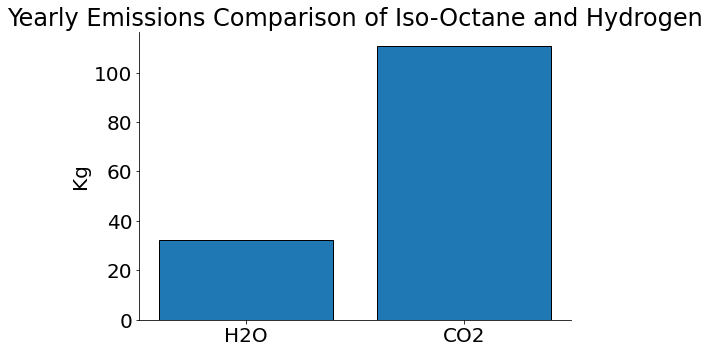
\includegraphics[width=1\textwidth]{Figures/Y_emiss_update.png}
    \caption{}
    \label{fig:code}
\end{figure}

When calculating the yearly emissions of a hydrogen combustion-powered engine with its gasoline-powered counterpart several key assumptions were made. We assumed the engine had an average operating speed of 3,000 rpm, and was driven for 30 minutes a day for 70 percent of the days in a year. Using mole ratios from the combustion reaction, yearly emissions were calculated using a known mass of combustion fuel per cycle at 25 percent stoichiometric ratios. The figure compares carbon dioxide emissions from iso-octane combustion to water emissions from hydrogen combustion. Final calculations reveal that under ideal conditions the same engine would produce 32.16 kg of water by combusting Hydrogen gas, and 110.97 kg of carbon dioxide by combusting iso-octane. It is also worth noting that iso-octane combustion also produces water, though this is excluded from the plot to emphasize the mass of carbon dioxide produced.

%balanced chemical formula

\subsubsection{Hydrogen-Oxygen Otto Cycle}
Hydrogen Oxygen combustion is a chemical reaction involving two moles of molecular hydrogen per mole of molecular oxygen, and results in two moles of water in addition to copious amounts of thermal energy. The reaction can be seen in Equation \ref{eq:combust}. It is this thermal energy which we exploit to produce work.

\begin{equation}
\label{eq:combust}
    2\text{H}_2 + \text{O}_2 \Rightarrow 2\text{H}_2\text{O}
\end{equation}

Hydrogen is a good candidate for internal combustion engines due to its very high heating value relative to other fuels, partially making up for its low density. This fact can be seen in Table \ref{tab:heating_vals}, where Hydrogen has around 2.5 times the lower heating value of Iso-octane. Of note, we consider only the lower heating values throughout the calculations for this report. This is because lower heating values are measures of energy released from a chemical reaction where the produced water is entirely in a gaseous state. Certainly, we do not want liquid water within our engine, and even if we did, we would have to produce a method to extract that energy from the released steam.

\begin{table}[H]
    \centering
    \begin{tabular}{|c|c|c|}
    \hline
    Fuel & LHV [kJ/kg] & HHV [kJ/kg]\\ \hline
    Hydrogen &  120000 & 141800 \\ \hline
    Iso Octane & 47890 & 44430\\ \hline
    \end{tabular}
    \caption{Lower and Higher heating values of Hydrogen gas. \cite{class_notes}}
    \label{tab:heating_vals}
\end{table}

When analyzing the ideal Otto Cycle for a 2-stroke engine operating on pure hydrogen and air, we considered the same operating condition under which the engine is rated for maximum power in its original configuration. After our analysis, we concluded power outputs at 6000rpm, displayed in Figure \ref{fig:power_diag}, for both Hydrogen and Iso-octane powered cycles. The engine is normally rated to operate at 1.6 kW at the same rpm when running on gasoline under real-world conditions. Our values are theoretical, and no losses are considered. Additionally, we calculate the state points of the simulated hydrogen-oxygen cycle and compile them into a pressure-volume graph, pressure-temperature graph, and temperature-entropy graph, displayed in Figures \ref{fig:pv_diag}, \ref{fig:pt_diag}, and \ref{fig:ts_diag}. We also calculate expected runtimes at various conditions, visualized in Figures \ref{fig:runtime_duty} and \ref{fig:runtime_rpm}. These values are all calculated in Python using PYroMat, a free library for thermodynamics analysis.\cite{pyromat}

For these analyses, we assume the following:

\begin{enumerate}
    \item All Gasses are Ideal
    \item Full Combustion of Reactants
    \item Intake Conditions at STP
    \item Iso-Octane Powered Engine is an Ideal Air Engine
    \item Hydrogen powered Engine is Not and Ideal Air Engine
\end{enumerate}

All gasses are ideal. We assume all gasses to be ideal. This assumption is reasonable, considering that, for the gasses involved, we are significantly above the phase change point. Thankfully, we are also below the extreme temperatures at which the dissociation of molecular species dominates and begins to alter properties of the gasses involved.

Full combustion of reactants. We assume the full combustion of reactants in the combustion chamber. This is important as is simplifies the reaction taking place. It also explains the very high power ratings we get from our theoretical calculations. With full combustion, combustion temperatures are incredibly high, much higher than real-life engines. This assumption also means the combustion chamber is fully evacuated after every expansion, and is fully replenished with new, uncombusted gas. This is not the true operation of many engines, particularly two-strokes, which oftentimes want some portion of the exhaust gasses to remain in the combustion chamber as a way to increase fuel-efficiency.

 Intake conditions at STP. We assume the gasses are at standard temperature and pressure at the intake. This may not necessarily be true for engines in the real world. Some may boost their pressures above ambient before compression. For example, many two-stroke engines use the downstroke of the piston to slightly compress the air-fuel mixture in the cranckcase, pushing it into the combustion chamber. Other engines may use a vacuum to pull air into the combustion chamber, and as a result operate with intake pressures below ambient. This is not complex to model or account for, but we have to base our intake on some value we know (STP) instead of some random intake pressure which may vary from engine to engine.

Iso-Octane powered Engine is an ideal air cycle. We are dealing with iso-octane in the liquid form, so its volume is considered negligible. Throughout the cycle, this may change. However, due to the high density of iso-octane and relatively low volume it would take up, we feel comfortable treating the iso-octane example as an air engine. During combustion, we add the heat of combustion from the iso-octane which would be required for combustion at the given fuel-air ratio.

Hydrogen powered engine is not an ideal air cycle. We know hydrogen makes up a significant portion of the volume of the intake gas. This is true due to the fact we need twice the moles of hydrogen as oxygen present in atmospheric gas for stoichiometric combustion. However, this means that many properties of air, such as specific heats, will change. We account for this in our calculations. This also means that, since hydrogen takes up lots of volume, the amount of oxygen present in the combustion chamber is less than that of the iso-octane powered engine. We also assume the composition of the exhaust gasses remains the same as the intake gasses, just as with the iso-octane powered engine analysis. For gas properties such as specific heats in the hydrogen-powered cycle, we take the weighted average of the corresponding properties from each gas. We re-calculate thee properties at every state point, due to the high fluctuation of specific heats of hydrogen.

Figure \ref{fig:power_diag} demonstrates that with fuel-air ratios lower than stoichiometric, we see a corresponding decrease in performance. This is expected behavior, and signals a large decrease in combustion temperatures.

\begin{figure}[H]
\centering
\begin{subfigure}{0.5\linewidth}
  \centering
  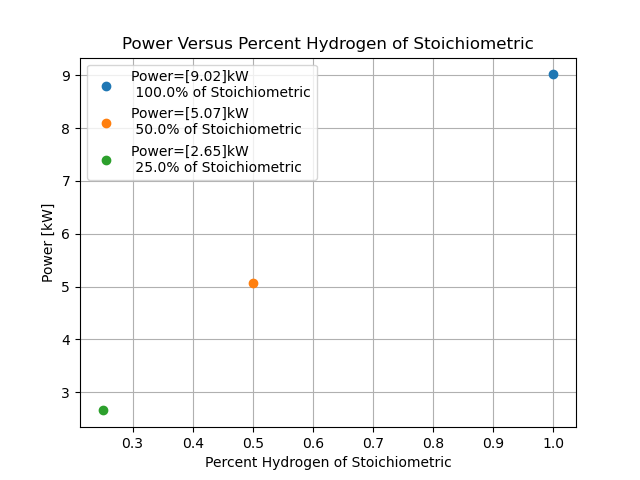
\includegraphics[width=1\linewidth]{Figures/Hydrogen/power_v_e.png}
  \caption{Hydrogen-air Otto cycle power diagram.}
  \label{fig:power_diag_h2}
\end{subfigure}%
\begin{subfigure}{0.5\linewidth}
  \centering
  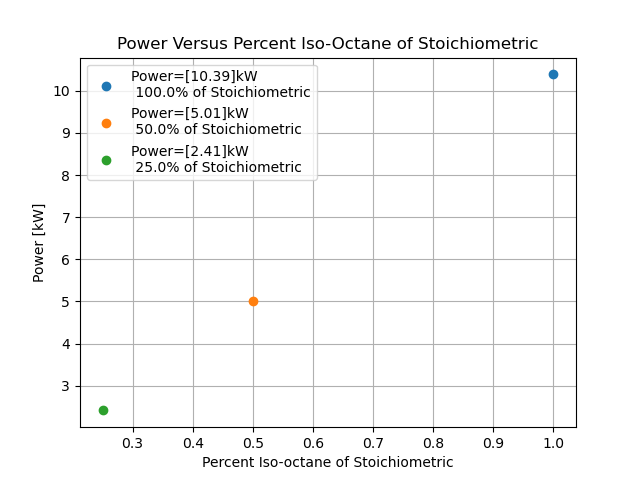
\includegraphics[width=1\linewidth]{Figures/Iso-octane/power_v_e.png}
  \caption{Iso-octane Otto cycle power diagram.}
  \label{fig:power_diag_iso}
\end{subfigure}
\caption{Power rating calculated in Python using a widely available thermodynamics library, showing ideal power out to percent of Hydrogen or iso-octane present compared to stoichiometric.}
\label{fig:power_diag}
\end{figure}

Figure \ref{fig:pv_diag} is the pressure-specific volume plot of our Otto cycle. Notably, the hydrogen system produces higher temperatures, higher specific volumes, and has shifting specific volumes per statepoint depending on the composition of the combustion gas mixture. These properties are the result of hydrogen having a much higher heat of combustion and lower density, while the gas mixture has thermal gas properties which fluctuate based on the amount of hydrogen present.

\begin{figure}[H]
\centering
\begin{subfigure}{0.5\linewidth}
  \centering
  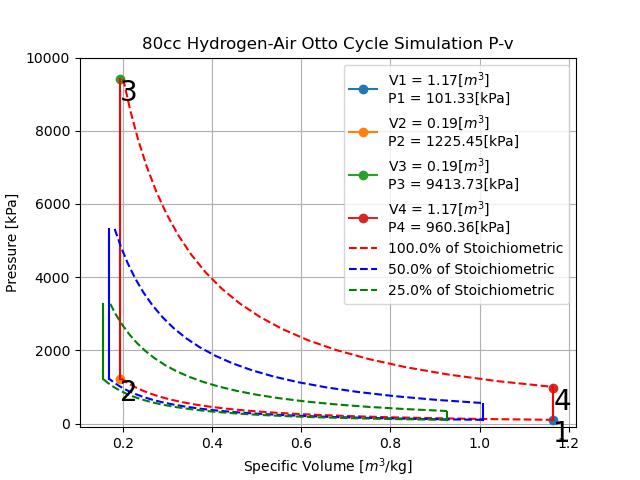
\includegraphics[width=1\linewidth]{Figures/Hydrogen/P-V_specific.png}
  \caption{Hydrogen-air Otto cycle P-v diagram.}
  \label{fig:p-v_diag_h2}
\end{subfigure}%
\begin{subfigure}{0.5\linewidth}
  \centering
  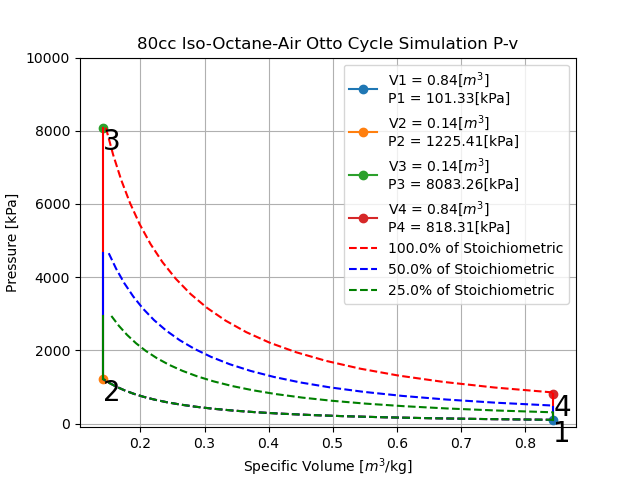
\includegraphics[width=1\linewidth]{Figures/Iso-octane/P-V_specific.png}
  \caption{Iso-octane Otto cycle P-v diagram.}
  \label{fig:p-v_diag_iso}
\end{subfigure}
\caption{Pressure versus specific volume state points of a simulated Hydrogen-Oxygen and Iso-octane Otto Cycle, at various fuel ratios.}
\label{fig:pv_diag}
\end{figure}

Figure \ref{fig:pt_diag} reveals the immmense impact the higher heat of combustion of hydrogen has on the overal system. At stoichiometric ratios and perfect combustion, hydrogen produces combustion temperatures far exceeding those of iso-octane. Reducing the amount of fuel available for combustion drasticaly reduces the temperatures of both systems, however hydrogen still manages to produce higher temperatures.

\begin{figure}[H]
\centering
\begin{subfigure}{0.5\linewidth}
  \centering
  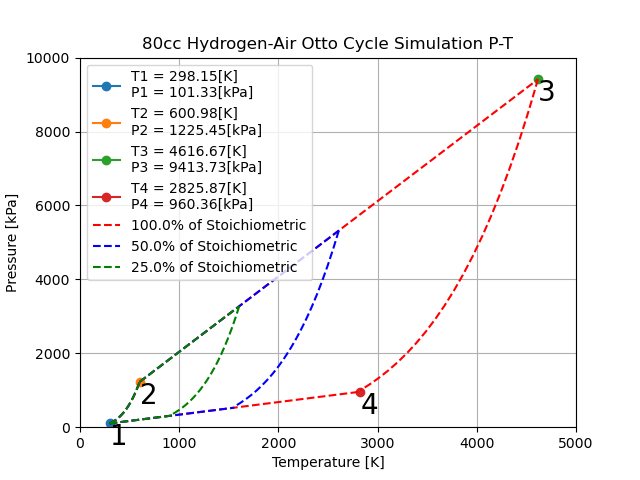
\includegraphics[width=1\linewidth]{Figures/Hydrogen/P-T.png}
  \caption{Hydrogen-air Otto cycle P-T diagram.}
  \label{fig:p-t_diag_h2}
\end{subfigure}%
\begin{subfigure}{0.5\linewidth}
  \centering
  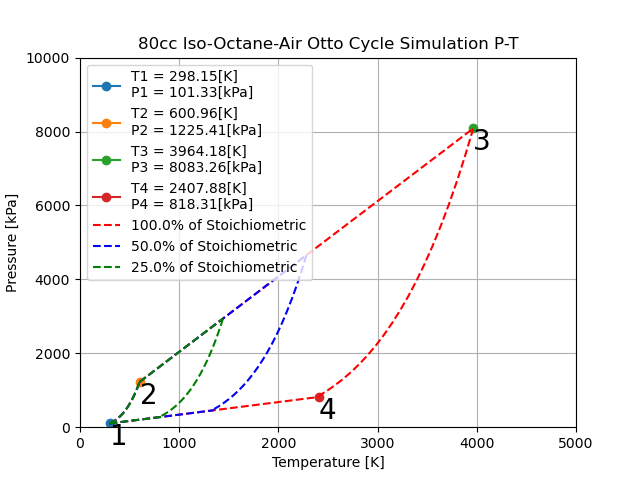
\includegraphics[width=1\linewidth]{Figures/Iso-octane/P-T.png}
  \caption{Iso-octane Otto cycle P-T diagram.}
  \label{fig:p-t_diag_iso}
\end{subfigure}
\caption{Pressure versus temperature state points of a simulated Hydrogen-Oxygen and Iso-octane Otto Cycle, at various fuel ratios.}
\label{fig:pt_diag}
\end{figure}

Figure \ref{fig:ts_diag} shows the unique impact our analysis of the hydrogen-powered cycle has on the calculated entropies. While the change in entropy from one state to another remains comparable between hydrogen and iso-octane, the antropy value at each point varies in the hydrogen example. This is due to the varying composition of the gas mixture. As this mixture approaches almost pure air, its entropy values close in on the values present in the air-engine model of the iso-octane powered cycle.

\begin{figure}[H]
\centering
\begin{subfigure}{0.5\linewidth}
  \centering
  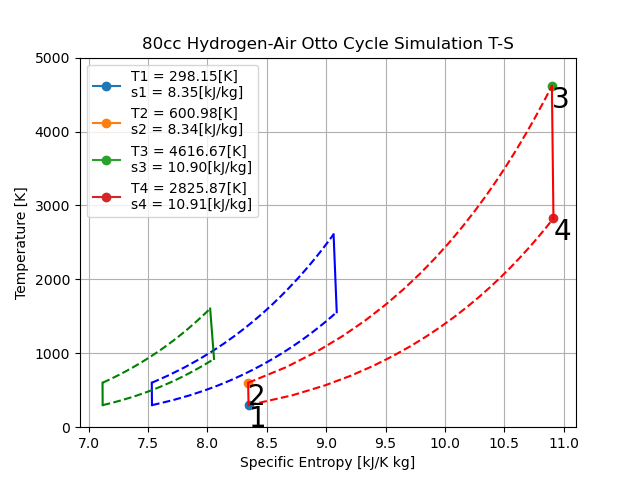
\includegraphics[width=1\linewidth]{Figures/Hydrogen/T-S.png}
  \caption{Hydrogen-air Otto cycle T-S diagram.}
  \label{fig:t-s_diag_h2}
\end{subfigure}%
\begin{subfigure}{0.5\linewidth}
  \centering
  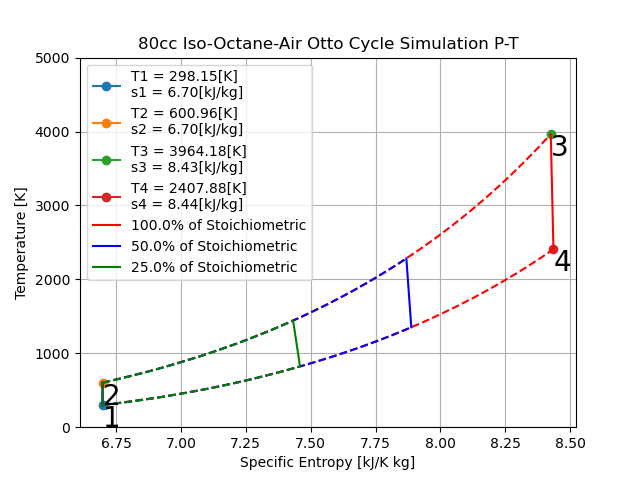
\includegraphics[width=1\linewidth]{Figures/Iso-octane/T-S.png}
  \caption{Iso-octane Otto cycle T-S diagram.}
  \label{fig:t-s_diag_iso}
\end{subfigure}
\caption{Temperature versus entropy state points of a simulated Hydrogen-Oxygen and Iso-octane Otto Cycle, at various fuel ratios.}
\label{fig:ts_diag}
\end{figure}

Finally, Figures \ref{fig:runtime_duty} and \ref{fig:runtime_rpm} showcase the different runtimes available with each system. We base the volume of the iso-octane system off of an approximate estimate of the tank sizes seen in similar two-stroke bicycle engine kits. Meanwhile, we base the hydrogen tank size off of the larges commercially available tanks that are still manageable on a small transport vehicle. These two graphs showcase one of the few weaknesses of hydrogen combusting systems. That is, hydrogen features very low specific energy when compared to other fuels, such as iso-octane. This is particularly apparent when hydrogen is still in a gaseous form. This means that the hydrogen-powered system is limited in range or runtime when compared to iso-octane.

\begin{figure}[H]
\centering
\begin{subfigure}{0.5\linewidth}
  \centering
  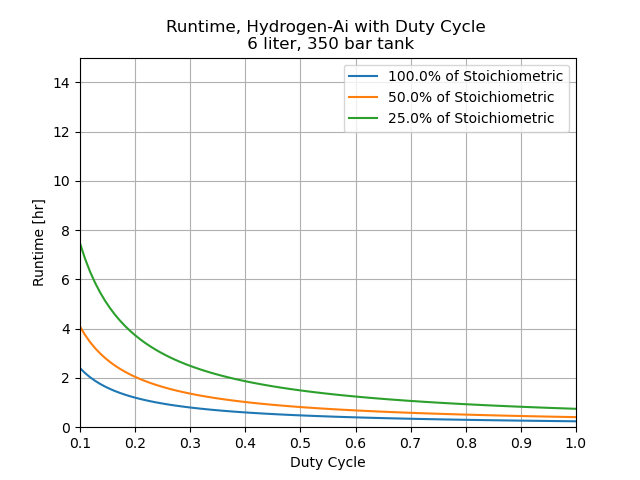
\includegraphics[width=1\linewidth]{Figures/Hydrogen/runtime_duty_cycle.png}
  \caption{Hydrogen-air Otto cycle runtime over duty cycle.}
  \label{fig:runtime_duty_h2}
\end{subfigure}%
\begin{subfigure}{0.5\linewidth}
  \centering
  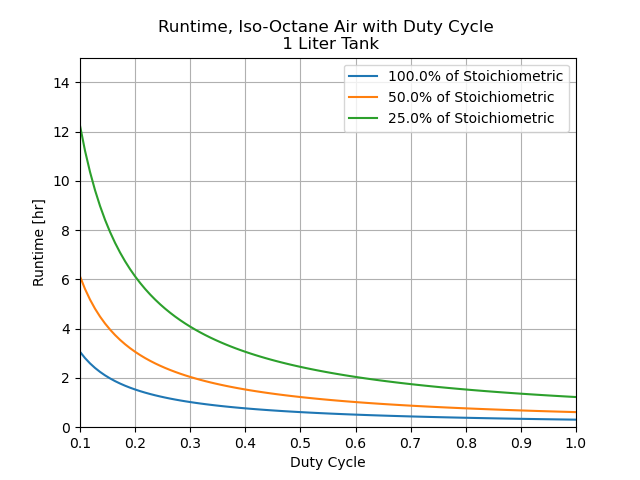
\includegraphics[width=1\linewidth]{Figures/Iso-octane/runtime_duty_cycle.png}
  \caption{Iso-octane Otto cycle runtime over duty cycle.}
  \label{fig:runtime_duty_iso}
\end{subfigure}
\caption{Runtimes of a simulated Hydrogen-Oxygen and iso-octane Otto Cycle, at 6000 RPM and various duty cycles. This data may be compared to real world usage to draw better conclusions on range and runtime.}
\label{fig:runtime_duty}
\end{figure}

\begin{figure}[H]
\centering
\begin{subfigure}{0.5\linewidth}
  \centering
  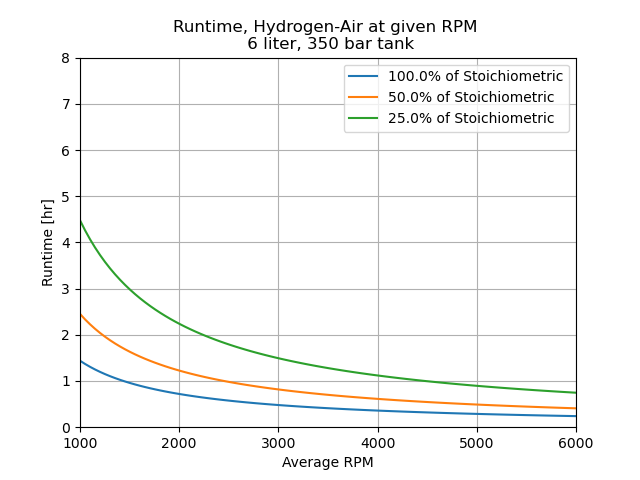
\includegraphics[width=1\linewidth]{Figures/Hydrogen/runtime_rpm.png}
  \caption{Hydrogen-air Otto cycle runtime over RPM.}
  \label{fig:runtime_rpm_h2}
\end{subfigure}%
\begin{subfigure}{0.5\linewidth}
  \centering
  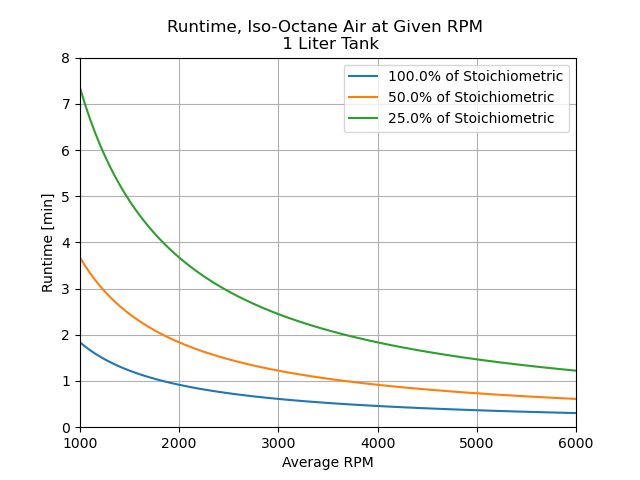
\includegraphics[width=1\linewidth]{Figures/Iso-octane/runtime_rpm.png}
  \caption{Iso-octane Otto cycle runtime over RPM.}
  \label{fig:runtime_rpm_iso}
\end{subfigure}
\caption{Runtimes of a simulated Hydrogen-Oxygen and iso-octane Otto Cycle, at 100 percent duty cycle over various RPMs. This data may be compared to real world usage to draw better conclusions on range and runtime.}
\label{fig:runtime_rpm}
\end{figure}

\subsection{Conversion Modifications}
%hydrogen and oxygen tank - can adapt existing tech like from welders for the tubing
%throttle with ball valve thing
%
Conversion of one of these engines could be done rather simply, as it could be adapted to intake the gas mixture using existing components that are used in pressurized systems like welders. The engine intake is threaded such that pressurized lines may be attached to it directly. The pressure and flow rate of the gases at the inlet may be controlled through the use of a pressure-reducing regulator such as those used in welding applications. These regulators are widely commercially available and are able to self-regulate to a desired flow rate while maintaining a desired pressure. These regulators would allow for a consistent gas mixture while allowing for variable flow rates, and maintaining throttle control of the engine. Additionally, a check valve would need to be placed in the system between the intake and the pressurized tanks to ensure safety in the event of an engine backfire.

Converting a 2-stroke engine such as this one poses difficulties when considering lubrication, however. A conventional 2-stroke engine relies on a mixture of oil and fuel to lubricate the internal components as intake gases are drawn through the crankcase. Oil could of course be atomized into the intake gas mixture, but this would again result in the combustion of hydrocarbons. Although a direct conversion of this existing engine to a sealed oil system would prove difficult, several solutions may prove feasible. An oil squirter system, such as is common on larger 2-stroke engines, may be implemented to more directly lubricate components and mitigate the amount of oil that enters the combustion chamber. A development in dry lubricants such as graphite may prove useful in solving this as well. Furthermore, a slightly more complex 2-stroke engine, such as those in marine applications with a packing seal that completely separates the crankcase and combustion chamber, could altogether avoid the issue of needing to combust hydrocarbons in the process of lubrication.
\section{Analysis}
\subsection{Materials}

\subsubsection{Pressure Vessel Materials}
Hydrogen presents an interesting engineering challenge due to its inherent qualities. The element, and its stable molecule $\text{H}_2$, are exceedingly small. So small, in fact, that that hydrogen can go into and through the metal lattice of its containing structure. This means that, over time, hydrogen will leak through an otherwise perfectly sealed pressure vessel. Additionally, the hydrogen can also remain within the lattice structure of the metal it interacts with. Over time, more and more hydrogen will diffuse into the metal, altering its mechanical properties. This process is called hydrogen embrittlement, and drastically lowers the tensile strength of the metal it diffuses into. Observing this process is incredibly difficult, as researchers at MIT have discussed, so knowing the extent to which some material is embrittled at a given point in time is difficult. \cite{MITNews:h2}. Thus, when storing hydrogen in a gaseous form within a pressure vessel, this is cause of concern, particularly if this is long term storage undergoing cyclical loading.

To mitigate this issue, we recommend storing hydrogen in containers approved for that purpose. However, this may not be a possibility in many parts of the world, in which case hydrogen should be stored at pressures significantly lower than what the container is rated for. This would leave enough margin in the case of full hydrogen saturation of the metal lattice of the container. Further research can be done to model common metals used in common types of pressure vessels, such as oxygen, argon, and carbon dioxide tanks, and their reactions to hydrogen embrittlement, as well as the resultant maximum tensile strength.

\subsubsection{Engine Materials}
Hydrogen embrittlement may also impact the materials used in the engine itself. Indeed, it is typical to use materials such as cast iron to forge the types of engines we are analyzing for conversion, and cast iron is particularly susceptible to hydrogen embrittlement. This is definitely not desirable, since the engine undergoes thermal stresses and vibrations on top of the pressure stresses generated from combustion and the cyclical loading of using an engine. All of these factors combined may cause cracks to form and propagate throughout the structure of the engine. Specifically, hydrogen reduces the strain and time to fracture, and plastic deformation occurring during hydrogen uptake increases the rate of hydrogen uptake. This is all according to Sahiluoma et. al, who also found that, at elevated temperatures hundreds of degrees above room temperature, cast iron may begin a desorption process where hydrogen leaves the lattice structure.\cite{Hydrogen_embrittlement_of_nodular_cast_iron} Hydrogen desorption in cast iron is visualized in Figure \ref{fig:cast_iron} as a function of temperature, where we can see desorption peak at around 480 and 640 degrees Kelvin. This means that, depending on the surface temperatures of the combustion chamber, hydrogen embrittlement may not be an issue within the engine, reducing the worry of fractures forming into cracks throughout the engine structure. This proves promising in allowing for simple, lasting conversions of existing internal combustion engines. However, more research needs to be done to draw conclusive results for our application.

\begin{figure}[H]
    \centering
    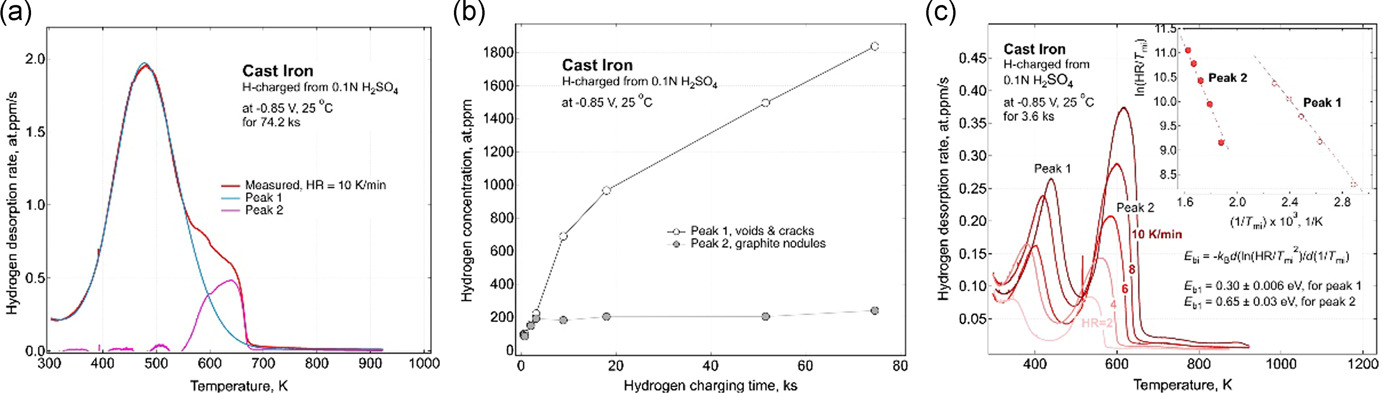
\includegraphics[width=1\textwidth]{Figures/desorpt.jpg}
    \caption{Hydrogen desorption in cast iron as a function of temperature.\cite{owidco2andgreenhousegasemissions:by_sector}}
    \label{fig:cast_iron}
\end{figure}

\subsection{Economics}
The largest economic consideration in this conversion kit is not the material or development cost of the static components of the kit like the tank(s), regulators, or tubing, but instead the availability, or lack thereof, of accessible hydrogen supply, which varies from serviceable in certain parts of the world to non-existent in others.  The validity of this kit as a realistic market product hinges on improvements being made in both this stated availability issue and the individual user's ability to electrolyze their own hydrogen supply; however, recent strides have been and are being made to work towards remedy of these issues.  For example, the Love's gas station chain has committed to adding hydrogen as a purchasable fuel option at its locations \cite{loves}, and recent electrolyser systems have been developed that are around a quarter the size of legacy models but achieve the same output.  If said systems can reach the point of feasible integration into the average home via domestic electrical grid power, users could produce their own fuel for their vehicle with the main cost being one of electricity usage.

\subsection{Social Impact}
While our proposed conversion system offers economic benefits , it may also contribute to a wide social impact in the adoptive countries. In the Global North, we oftentimes take perceived advances in our society for granted. Take for example Norway. The nation is world renowned for its high human development, per capita gdp, and, interestingly, its breakneck adoption of electric vehicles. In 2022, 80 percent of the nation’s automobile sales were electric vehicles \cite{norway}. On the surface, this seems like an incredible achievement, as a problem solved only by the wise policies of the Norwegian government, which heavily subsidize electric vehicle purchases, and which should be replicated everywhere. However, these policies were only possible due to several factors unique to Norway and the Global North in general.

Countries in the Global North are wealthy enough to afford decarbonization. They have established institutions, large budgets, and the political capital necessary not only to debate the act of making their societies greener, but to actually implement and execute those ideas. Nations in the global south are at a comparative disadvantage. They do not have the funds to subsidize large industrial sectors, if they even exist. They do not have the institutions to monitor and encourage adoption of green technologies. And if they were to adopt green technologies on a mass scale, the manpower needed to install and safely operate these technologies may not exist. To start a zero-emissions industrial park in the global south in many cases means building the industrial facilities and all of the associated green infrastructure. In places like the U.S., oftentimes it's just a matter of buying carbon credits.

The proposed conversion system may help less developed countries achieve better rates of environmental sustainability without the need for strong, preexisting institutions or centralized directives backed by large subsidies. Instead, if conversion technology such as the one proposed is made cheap, widely available, and simple enough to penetrate large regions of the world without advanced technical knowledge, individuals and small groups can take matters into their own hands by transforming their personal transportation vehicles. This sidesteps the need for a strong central bureaucracy to incentivize green developments.

These small changes happening millions of times with the help of billions of people have the potential to crate a large impact. It can provide motorized transportation to remote areas, as one would not need to be connected to a central grid or gas distribution system to operate this proposed converted machinery (Solar concentrator stirling engine, converted motor, gas storage). It could help promote nascent native industries, promote responsible consumption and production, propagate affordable and clean energy, create more sustainable communities, and better the environment through reduced pollution. All of these potential effects can be associated with the United Nations Sustainable Development Goals Numbers 7, 8, 9, 11, 12, and 13, which are:

\begin{itemize}
    \item Affordable and Clean Energy
    \item Decent Work and Economic Growth
    \item Industry, Innovation, and Infrastructure
    \item Sustainable Cities and Communities
    \item Responsible Consumption and Production
    \item Climate Action
\end{itemize}

These and the rest of the goals can be found under the United Nations Department of Economic and Social Affairs. \cite{un_sdg}

\section{Conclusion}
If sufficient advancements are made in the near-future in the hydrogen storage, production, and supply space, which industry trends are indicating as more and more realistic each year, this proposed conversion kit for a petrol powered bicycle engine to be swapped to hydrogen as its combustible fuel would allow for a relatively straightforward way for owners of said vehicles to practically eradicate the direct carbon footprint of their chosen method of transportation and, with the realization of small scale electrolysis technology, save money as well.  Additionally, while at the moment much of the world's electricity is still generated via coal burning and natural gas combustion, as we transition more and more to renewable means of energy production each year, the power required to produce electrolysis is less and less of a blemish on an otherwise emissions-free transportation method.


\section*{Appendix}

\subsection{CODE}

Code and calcualted results for this project can be found on Arturo's github repository.\cite{Saucedo_ME400_MP3_Software_2023}

\section*{Acknowledgments}
We would like to thank Dr. Christopher R. Martin, Associate Professor of Mechanical Engineering from The Pennsylvania State University for creating and distributing the free PYroMat python thermodynamics library. His contributions to making thermodynamics analysis software free and easily available for all were of great benefit to us and our project.

\bibliography{sample}

\end{document}
